\subsection{MetaQC}
For MetaQC, we used prostate cancer datasets with 8 datasets.
??Decide if we need more description here??

\subsubsection{Merging}

The datasets from all the 8 studies (uploaded in ``Preprocessing" step and named as ``p1.csv", ``p2.csv", etc.) should be merged before implementing MetaQC tool (Figure \ref{fig:merge}). The genes with low mean or low variance were filtered out (by default, the lowest 30th percentiles). Detailed information can be found in the ``preproc" package in the metaOmics software suite (\url{https://github.com/metaOmic/preproc}).

\begin{figure}[H]
\begin{center}
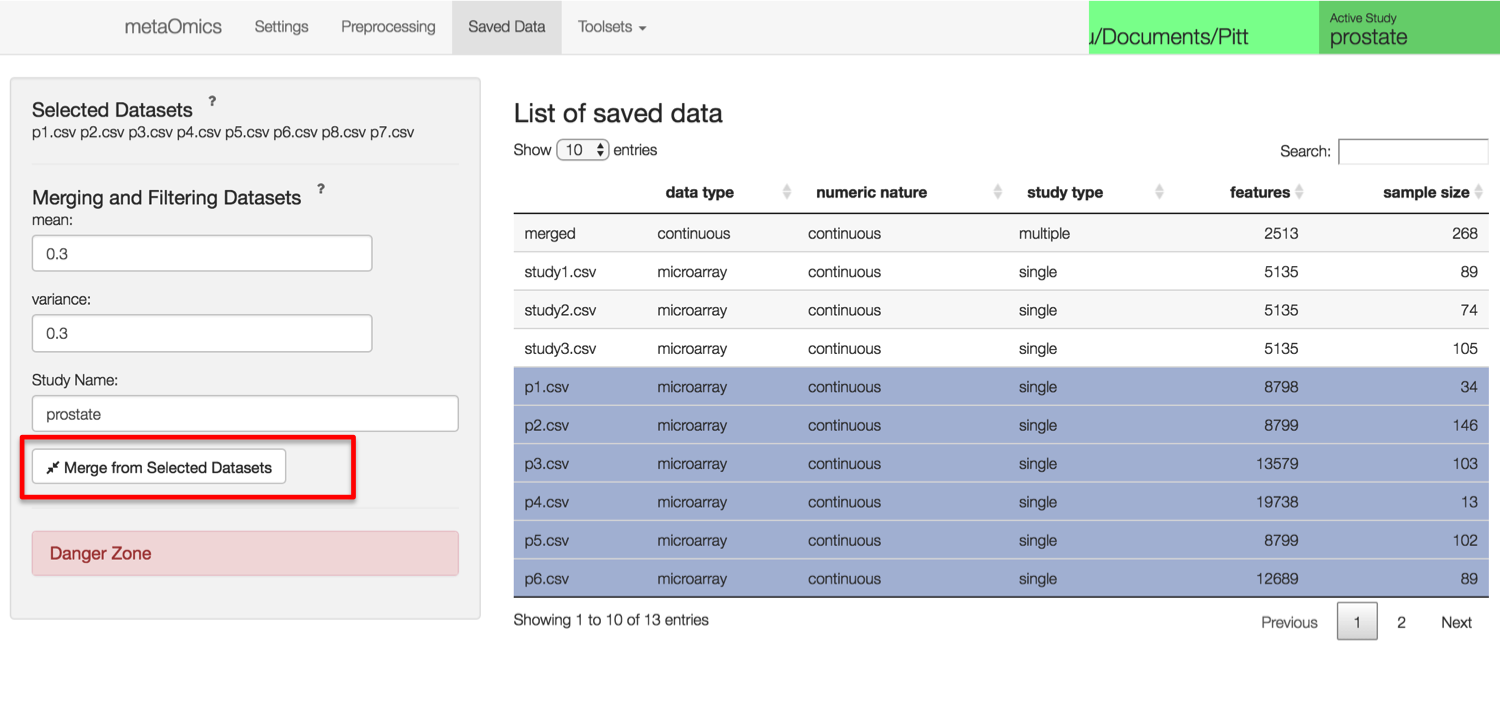
\includegraphics[scale=0.4]{./figure/metaQC/merge2}
\caption{Merging data for meta-analysis}
\label{fig:merge}
\end{center}
\end{figure}

\subsubsection{MetaQC analysis}

After opening the MetaQC page, as shown in Figure \ref{fig:MetaQCmainpage}, there are 2 tabs on the left of the page (``Options" and ``Advanced Options"). We generally suggest users not to change any parameter setting in the ``Advanced Options" unless users know the underlying methodology well. 

\begin{figure}[H]
\begin{center}
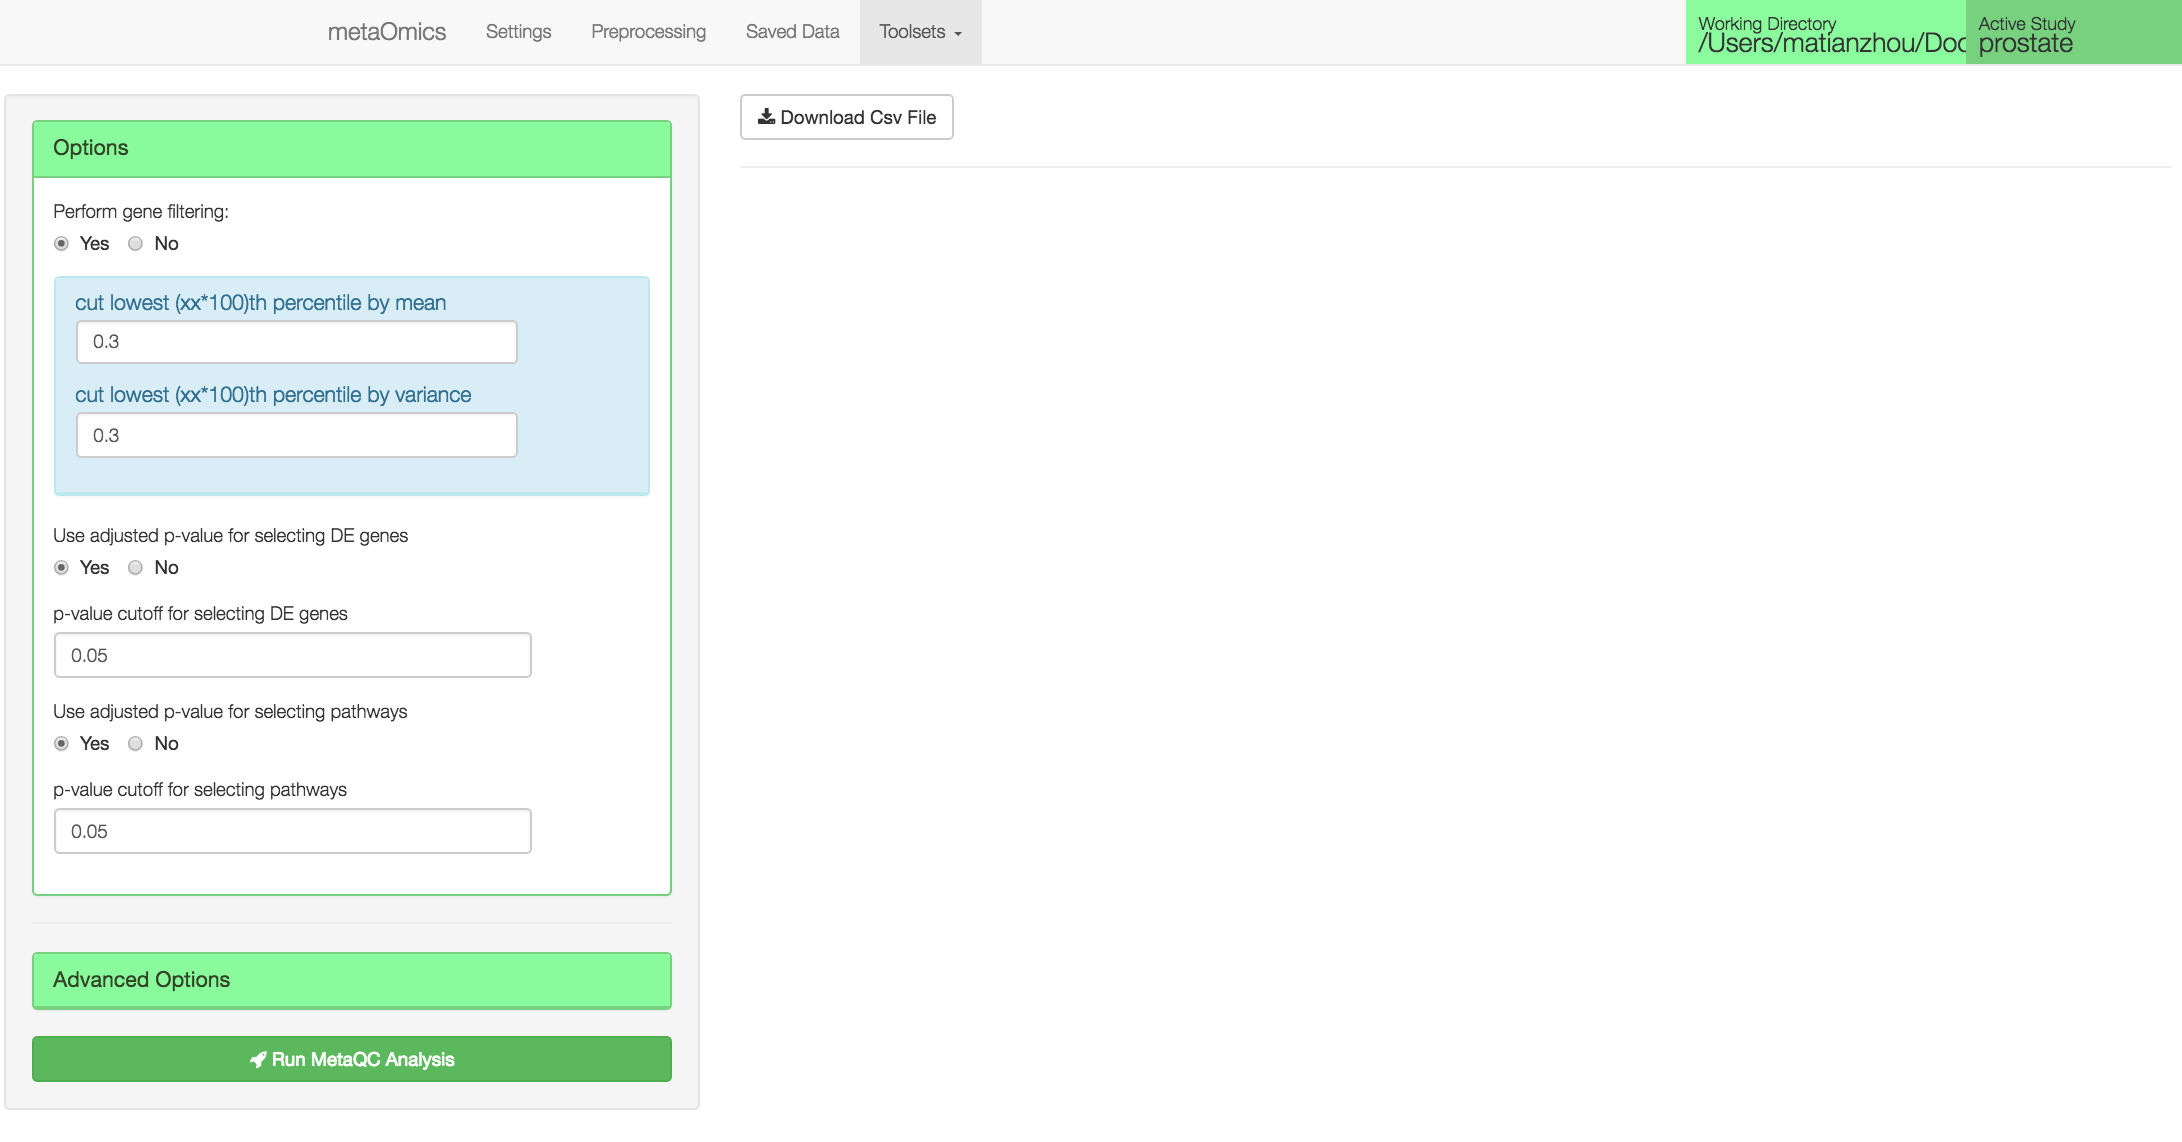
\includegraphics[scale=0.5]{./figure/metaQC/MetaQCmainpage}
\caption{Homepage of MetaQC}
\label{fig:MetaQCmainpage}
\end{center}
\end{figure}

For the current dataset, we already performed filtering while merging the 8 studies so we do not further filtered genes here and chose  ``No" for gene filtering (Figure \ref{fig:option1}). Moreover, MetaQC method requires users to choose a cutoff to decide significant DE genes and a cutoff to decide significantly enriched pathways, there are four options available, i.e. p-value cutoff for selecting DE genes, whether to use adjusted p-value or selecting DE genes, p-value cutoff for selecting pathways, whether to use adjusted p-value or selecting pathways. These options can be tuned depending on the overall signal of the datasets. Here, we use the defaults as determined by the prostate data.   

\begin{figure}[H]
\begin{center}
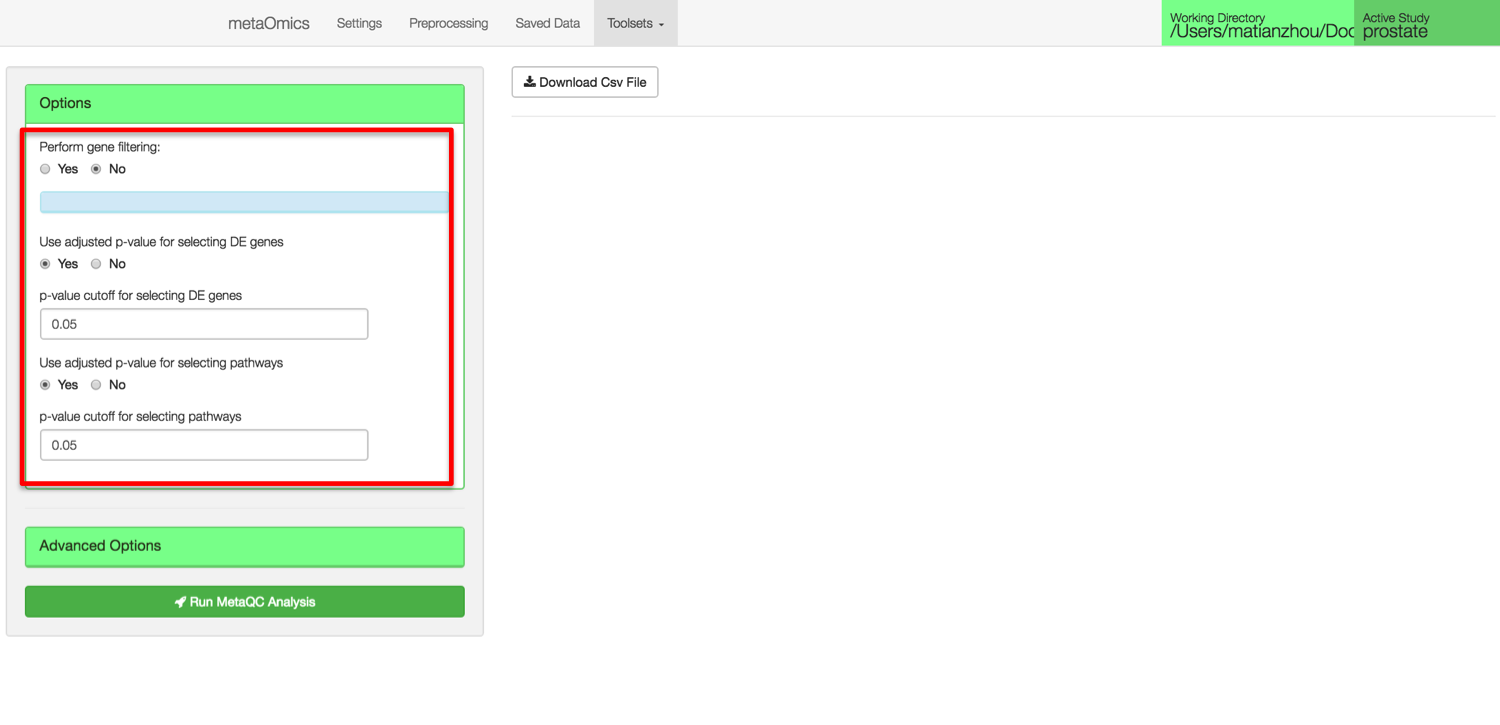
\includegraphics[scale=0.5]{./figure/metaQC/option1}
\caption{MetaQC Options}
\label{fig:option1}
\end{center}
\end{figure}

** Optionally, we can click on ``Advanced Options", choose ``min pathway size" and ``max pathway size" to include only pathways of reasonable size. We suggest 100 permutations is sufficient, and generally do not recommend users to change the number of permutations here (Figure \ref{fig:option2}). 

\begin{figure}[H]
\begin{center}
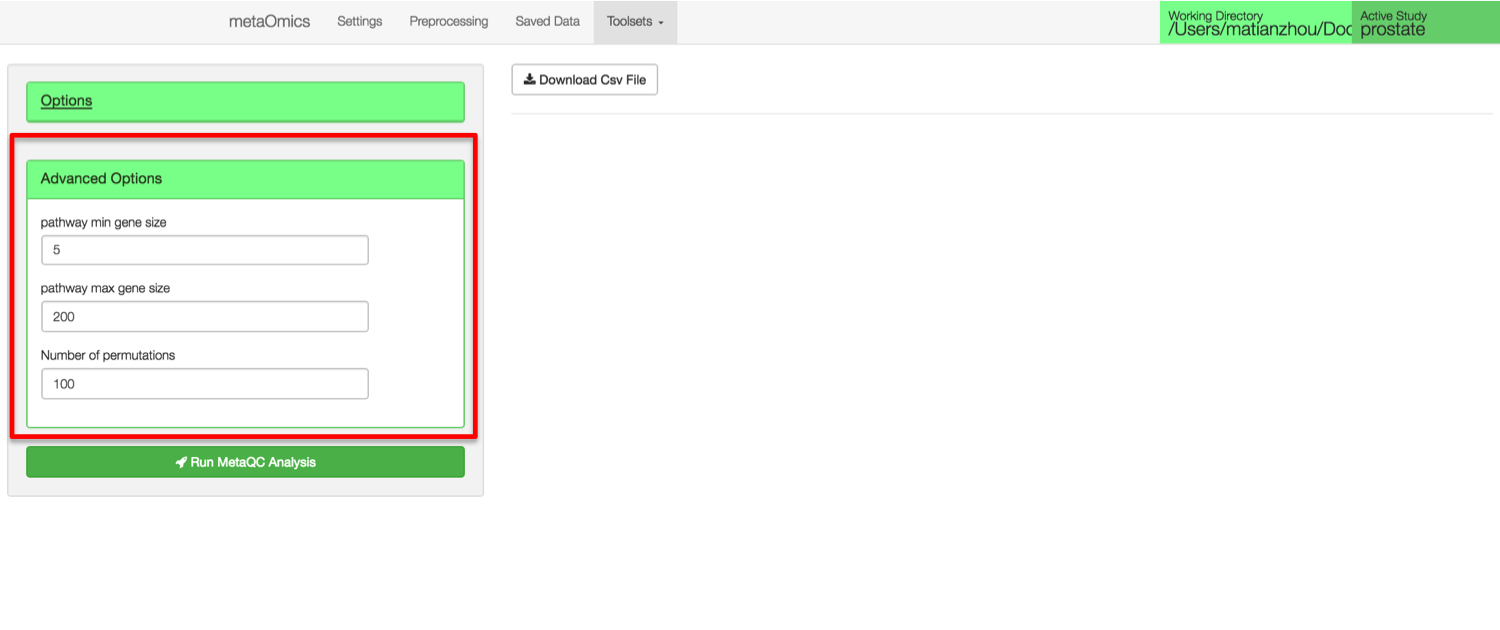
\includegraphics[scale=0.5]{./figure/metaQC/option2}
\caption{MetaQC Advanced Options}
\label{fig:option2}
\end{center}
\end{figure}

After we click on ``Run", we will see a summary table of MetaQC generated on the right of the page as shown in Figure \ref{fig:result}. The table includes seven columns, with the first six columns corresponding to the six quantitative quality control measures of all studies (a larger value indicates a better quality) and the seventh column is the rank summary statistics of all the six quality measures (a lower rank indicates a better quality). Users can download the full table as a csv file by clicking on ``Download Csv File". In addition to the tabular results, the tool also generated a PCA biplot from the six quality control measures, where the circled number is the study index and arrows indicate different measures (Figure \ref{fig:result}). Both tabular summary and biplot are automatically saved to the current working directory. 

\begin{figure}[H]
\begin{center}
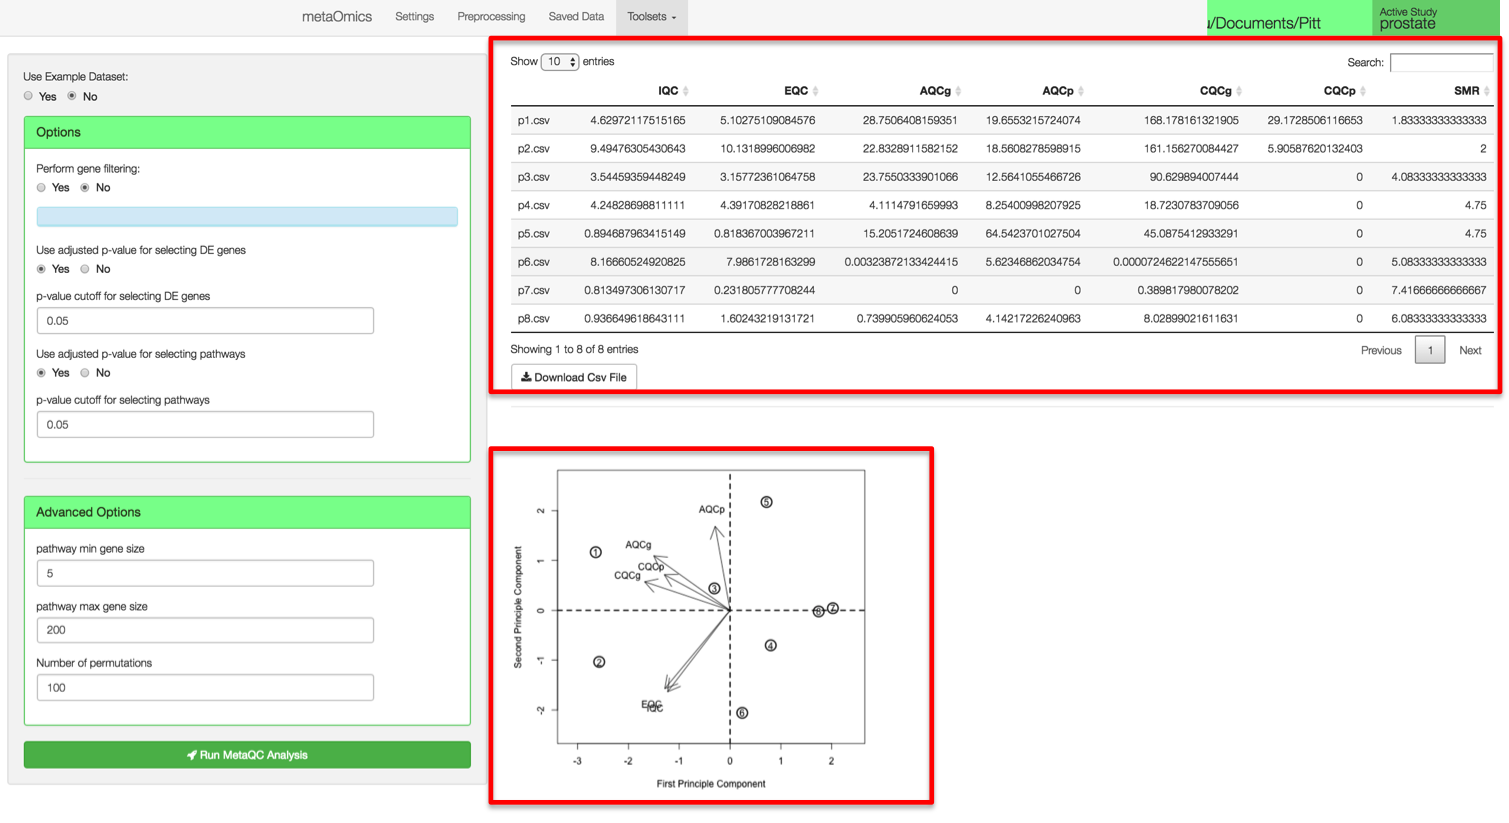
\includegraphics[scale=0.5]{./figure/metaQC/result}
\caption{MetaQC results: summary table and PCA biplot}
\label{fig:result}
\end{center}
\end{figure}


